\documentclass[11pt, handout]{beamer}
\mode<article> % only for the article version
{
  \usepackage{fullpage}
  \usepackage{hyperref}
%\usepackage[ps2pdf]{hyperref}
}
\usepackage{epsfig}
\usepackage{fancybox}
\usefonttheme[onlymath]{serif}

\mode<presentation>
{
%  \setbeamertemplate{background canvas}[vertical shading][bottom=white,top=blue!10]
%     \usetheme{Warsaw}
% \usetheme{CambridgeUS}
%  	\usetheme{Frankfurt}
%  	\usetheme{Berlin}
%  	\usetheme{Antibes}
%   \usetheme{Darmstadt}
%    \usetheme{Madrid}
%    \usefonttheme[onlysmall]{structurebold}
 	\usecolortheme{orchid}
% 	\usecolortheme{seahorse}
  \usecolortheme[named=blue]{structure}
% 	\usecolortheme{crane}
%	\usecolortheme{lily}
}

\setbeamercolor{math text}{fg=green!50!black}
\setbeamercolor{normal text in math text}{parent=math text}

\usepackage{color}
\usepackage{epsfig}
\usepackage{amsmath}
\usepackage{amssymb}
%\usepackage{beamerthemesplit}
\usepackage{listings}
 \lstset{language=Python,
    basicstyle=\ttfamily\bfseries,
    commentstyle=\color{red}\itshape,
  stringstyle=\color{green},
  showstringspaces=false,
  keywordstyle=\color{blue}\bfseries,
  breaklines=true,
%  postbreak=\mbox{\textcolor{red}{$\hookrightarrow$}\space},
  }
  
\usepackage[vlined,algoruled,titlenotnumbered,linesnumbered]{algorithm2e}
\usepackage{color}
\newcommand{\argmaxF}{\mathop{\mathrm{argmax}}\limits}


%\usepackage{lmodern}
%\usepackage[T1]{fontenc} 

\setlength{\leftmargini}{0pt}

\usepackage{times}

\setbeamercovered{dynamic}

\title[NLP]{Natural Language Processing}
\subtitle{Lecture IV. Part-of-speech (POS) tagging and Named Entity Recognition (NER)}
\author[Forrest Sheng Bao]{Forrest Sheng Bao, Ph.D.}
\institute[ISU]{Dept. of Computer Science \\ Iowa State University \\ Ames, IA 50011}
%\date[9/19/2017]{Sept. 19, 2017}

%\AtBeginSection[] {
%  \begin{frame}[plain]
%    \frametitle{Outline}
%    \tableofcontents[currentsection]
%  \end{frame}
%  \addtocounter{framenumber}{-1}
%}

\AtBeginSubsection[] {
  \begin{frame}[plain]
   \frametitle{Outline}
    \tableofcontents[currentsubsection]
    \addtocounter{framenumber}{-1}
  \end{frame}
} 

\begin{document}

 \frame{\titlepage}
 
 \section<presentation>*{Outline}
 
   \begin{frame}
     \frametitle{Outline}
  \tableofcontents
   \end{frame}

 
\section{What is POS tagging?}

\begin{frame}{POS}
\begin{tabular}{cccccccccc}
 \scriptsize Natural & \scriptsize Language & \scriptsize Processing &  is &  a & \scriptsize field &  of & \scriptsize computer & \scriptsize science.  \\
Adj. & n. & n. & v.  & dt. & n. & cj. & n. & n.
\end{tabular} 
 
\end{frame}


\begin{frame}{Part of speech tagging}
\begin{itemize}[<+->]
 \item ``In traditional grammar, a part of speech (abbreviated form: PoS or POS) is a category of words (or, more generally, of lexical items) which have similar grammatical properties. '' 
 \item ``In corpus linguistics, part-of-speech tagging (POS tagging or POST), also called grammatical tagging or word-category disambiguation, is the process of marking up a word in a text (corpus) as corresponding to a particular part of speech, 
 \item  based on both its definition and its context, i.e., its relationship with adjacent and related words in a phrase, sentence, or paragraph.'' 
 \item Brill tagger (circa. 1993): the first English POS tagger, rule-based. It assigns initial tags to words first and then use rules to iteratively  update tags based on, e.g., context. 
 \item Brill tagger has hundreds of rules. 
\end{itemize}
\end{frame}

\begin{frame}{Tags used in Penn Treebank}
 \begin{itemize}[<+->]
  \item Nine common parts of speech in English:  noun, verb, article, adjective, preposition, pronoun, adverb, conjunction, and interjection. 
  \item Most NLP researchers use Penn Treebank tags, which are finer than common English POSes mentioned above. 
  \item \url{https://www.ling.upenn.edu/courses/Fall_2003/ling001/penn_treebank_pos.html}
 \end{itemize}
\end{frame}

\begin{frame}{Why do we still need POS tagging? }
  \begin{itemize}[<+->]
    \item In DL era, models are end-to-end. Is POS tagging out of fashion? 
    \item There are still many cases where training data is not enough or labeling is very costly. 
    \item POS tags are a good intermediate feature, trained on large amounts of data. 
    \item The hidden states of POS taggers can be considered as a syntactical  representation of text. 
    \item One way to look at POS tagging is to treate is an NP-Complete problem. It's a bridge. 
    \item What's new today in NLP? Adept AI. 
  \end{itemize}
\end{frame}

\begin{frame}{Probabilistic Model for Tagging}

\begin{itemize}[<+->]
 \item Problem of using rule-based system: Very difficult to verify and to scale. 
 \item Probabilistic approach: there are many sequences of tags,  but only one yields (i.e., argmax) the highest probability. %Find the most likely one from all possible $\mathbf{T}$'s. 
 
%  \hskip -5em
 \begin{tabular}{cccccccccc}
~ &  \scriptsize Natural & \scriptsize Language & \scriptsize Processing &  is &  a & \scriptsize field &  of & \scriptsize computer & \scriptsize science.  \\
$\mathbf{T}_1$ & aj. & n. & n. & v.  & dt. & n. & cj. & n. & n. \\
$\mathbf{T}_2$ & n. & n. & n. & v.  & n. & n. & cj. & n. & n. \\
$\mathbf{T}_3$ & v. & n. & av. & v.  & dt. & n. & cj. & n. & n. \\
$\mathbf{T}_4$ & dt. & n. & n. & v.  & v. & n. & aj. & v. & n.\\ 
$\mathbf{T}_5$ & cj. & n. & n. & v.  & dt. & n. & cj. & n. & n.
\end{tabular} 
 
$\mathbf{T}_2$ - $\mathbf{T}_5$ apparently make no sense and hence their $P()$'s are very low. 
 

% ~
% \hskip -4em
% ~~~~~
% \begin{tabular}{cccccccccc}
% $\mathbf{W}$ & \scriptsize Natural & \scriptsize Language & \scriptsize Processing & \scriptsize is & \scriptsize a & \scriptsize field & \scriptsize of & \scriptsize computer & \scriptsize science.  \\
% $\mathbf{T}$ & JJ & NN & NN & VBZ  & DT & NN & IN & NN & NN.
% \end{tabular} 
% 
% \vskip 1em \pause



\item 
The goal is to find the most likely sequence of tags ($\mathbf{T}$), given the sequence of words ($\mathbf{W}$), i.e., 

$$
\argmaxF_\mathbf{T}  P(\mathbf{T}|\mathbf{W})
$$

\end{itemize}

\end{frame}


\section{POS tagging in HMM}

\begin{frame}{A generative model for POS tagging}
\begin{itemize}[<+->]


 \item Make use of Bayes' rule:

 \begin{align}
\argmaxF_\mathbf{T}  P(\mathbf{T}|\mathbf{W}) &= \argmaxF_\mathbf{T} \frac{P(\mathbf{W}|\mathbf{T}) P(\mathbf{T}) }{P(\mathbf{W})}  \\
       &= \argmaxF_\mathbf{T} P(\mathbf{W}|\mathbf{T}) P(\mathbf{T}) 
\end{align}
{\tiny Note that we go from Eq. (1) to Eq. (2) because $P(\mathbf{W})$ is not a function of $\mathbf{T}$.}

 \item tag-to-tag \textit{transition} probabilities: $P(\mathbf{T}) = \Pi_{i=1}^{l+1} P_T(t_i | t_{i-1}) $: e.g., \item the probability of the first tag sequence: $P(\mathbf{T_1}) = P_T(JJ|\rhd) \times P_T(NN|JJ)   \times P_T(NN|NN)  \times \cdots $.
 
 \item tag-to-word \textit{emission} probabilities: $P(\mathbf{W}|\mathbf{T}) = \Pi_{i=1}^{l} P_E(w_i|t_i) $: e.g., $ P(\mathbf{W}|\mathbf{T_1}) = P_E(``natural''|JJ) \times P_E(``language''|NN)  \times P_E(``processing''|NN)   \times \cdots $.

\end{itemize}
\end{frame}

\begin{frame}{A generative model for POS tagging}
  \begin{itemize}[<+->]
   \item A sequence of words is generated in two phases:
   \begin{enumerate}
    \item Produce a sequence of tags, e.g., $\rhd$, NN, DET, ..., based on probability between each two consecutive tags. 
    \item For each tag, produce a word, e.g., NN $\rightarrow$ ``language'', DT $\rightarrow$ ``the''. 
   \end{enumerate}
  
    \item Yes, a semantically meaningless sentence can be tagged and further parsed correctly,  e.g., ``NLP is a automobile of GOP''.
  \end{itemize}
  \end{frame}


\begin{frame}{}
  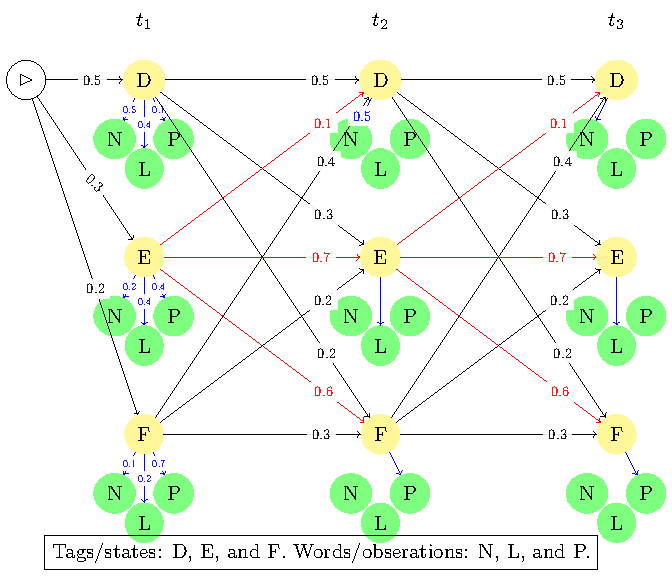
\includegraphics[width=\textwidth]{example.pdf}
\end{frame}


 \begin{frame}{A generative model for POS tagging}
% ~
% \hskip -4em
% ~~~~~
% \begin{tabular}{cccccccccc}
% $\mathbf{W}$ & \scriptsize Natural & \scriptsize Language & \scriptsize Processing & \scriptsize is & \scriptsize a & \scriptsize field & \scriptsize of & \scriptsize computer & \scriptsize science.  \\
% $\mathbf{T_1}$ & JJ & NN & NN & VBZ  & DT & NN & IN & NN & NN.
% \end{tabular} 

\begin{itemize}
 \item The generative model we just see is a typical Hidden Markov Model (HMM), where a tag is a \emph{state} and a word is an \emph{observation}. 
 \item In each state/tag, a word/observation emits. After each emission, transit to the next state/tag and emit a word/observation again. 
 \item Why Markovian?  The probably of a tag is only conditioned on the previous tag. No further history. First-order Markovian. 
 \item The transition and emission probabilities can be obtained by scanning the corpus once. 
\end{itemize}
\end{frame}

\begin{frame}{A generative model for POS tagging}
 \begin{itemize}[<+->]
%   \item Remember, we don't have the tag sequence, $\mathbf{T} = [t_1, \dots, t_l]$, i.e., the tag sequence is to be found out. 
  \item In principle, we just need to enumerate all possible tag sequences, $\mathbf{T}_1, \mathbf{T}_2, \dots$ and find the one that yields the largest  $P(\mathbf{W}|\mathbf{T}) P(\mathbf{T})$.
  \item But this is costly: If we have $N$ different tags and $l$ words in the sentence, there are $N^l$ possible/hidden tag sequences. 
  \item Smarter way? Viterbi algorithm -- a good example of dynamic programming. 
 \end{itemize}
\end{frame}

\begin{frame}[shrink]{HMM decoding in Viterbi algorithm}
\begin{itemize}[<+->]
 \item The problem of estimating the sequence of hidden states given a sequence of observations is known as \emph{decoding} in HMM. 
 \item Basic principle (Lemma 1): $\max(x\cdot y) = \max(x) \cdot y$,  if $x$ is a real variable and $y$ is a real constant. 
 \item In each step $i$ (except the start and end), we have $N$ possible states/tags $t_i$'s, each of which can come from $N$ possible $t_{i-1}$'s.  
%  $\Pi_{i=1}^{l-1} P_T(t_i|t_{i-1}) P_E(w_i|t_i)$'s and $N$ possible $P_T(t_l|t_{l-1}) P_E(w_l|t_l)$'s.
%  \item Suppose that there are $N$ possible states/tags. Then there are 
  \end{itemize} 
\end{frame}

\begin{frame}{Viterbi algorithm in math induction}
  \begin{itemize}[<+->]
    \item If the sentence has only one word: $\mathbf{W}= [w_1]$. The best tag  $t_1$ should  maximize $P_T(t_1|\rhd) P_E(w_1|t_1)$ where $\rhd=t_0$ is the beginning of the sentence. 
    % $\argmaxF_{t_1} . % Denote $P_T(t_1|\rhd)P_E(w_1|t_1)$ as $score(t_1)$. 
     \item If it has two: $\mathbf{W}= [w_1, w_2]$.  The best tags $t_1$ and $t_2$ shall maximize 
      $\Pi_{i=1}^{2} P_T(t_i|t_{i-1}) P_E(w_i|t_i)$ = $P_T(t_1|\rhd) P_E(w_1|t_1)  P_T(t_2|t_1) P_E(w_2|t_2)$. Just search over the $N^2$ combinations of $t_1$ and $t_2$, time complexity $O(N^2)$.
    \item If it has three: $\mathbf{W}= [w_1, w_2, w_3]$. \underline{Given tags $t_2$ and  $t_3$}, 
    \begin{align*}
    &  \max P_T(t_1|\rhd) P_E(w_1| t_1) P_T(t_2|t_1) P_E(w_2| t_2) & \overbrace{P_T(t_3|t_2) P_E(w_3| t_3)}^{\text{search only happens here}} \\
    = &  \left [   \max P_T(t_1|\rhd) P_E(w_1| t_1) P_T(t_2|t_1) P_E(w_2| t_2)  \right ]  & P_T(t_3|t_2) P_E(w_3| t_3)
    % \\
    % =  & ~~~~~~~~~~~~ v_{1,2}  &  P_T(t_3|t_2) P_E(w_3| t_3) 
    \end{align*}
    \item % Thus, to find the maximum when expanding from $t_2$ to $t_3$, we just need to search over $N^2$ products.
     No need to check $N^3$ combinations of tags $t_1$, $t_2$ and $t_3$, many of which will not maximize the final number regardless of the value of $P_T(t_3|t_2) P_E(w_3| t_3)$. Instead, check $N + 2N^2 \in \mathcal{O}(3N^2)$ combinations. 
  \end{itemize}
\end{frame}

\begin{frame}{HMM decoding in Viterbi algorithm}
\begin{itemize}[<+->]
 \item Let's generalize: 
 \begin{align*}
  &  \max \Pi P_T(t_i|t_{i-1}) P_E(w_i| t_i) & P_T(t_{i+1}|t_i) P_E(w_{i+1}| t_{i+1}) \\
  = &  \left [  \max \Pi P_T(t_i|t_{i-1}) P_E(w_i| t_i) \right ] & P_T(t_{i+1}|t_i) P_E(w_{i+1}| t_{i+1})
  \end{align*}
 \item Denote $v(\overbrace{i}^{\text{step or word index}}, \overbrace{j}^{\text{state or tag index}})$ as the probability that the HMM is in state $j$ after seeing the first $i$ observations and passing through \textbf{the most probable} preceding sequence of states. We call $v(i,j)$ the \emph{previous Viterbi path probability}. 
%  in order to maximize the entire chain $\Pi_{i=1}^l P_T(t_i|t_{t-1}) P_E(w_i|t_i)$, we just need to find the transition at each step that maximizes. 
 \item 
 $$
 v(i,j) = \max_{j=1}^N v(i-1, j)P_T(t_i|t_j) P_E(w_i|t_i)
 $$
 \item If we repeat this step by step, we can find the maximum $P(\mathbf{T}|\mathbf{W})$. 
 \item Then a traceback allows us to find the tags that maximizes it.
%  \item And, the ideal $t_i = \argmaxF_i v(i,j)$
 \end{itemize} 
\end{frame}

\begin{frame}{HMM decoding in Viterbi algorithm}
 \begin{itemize}
  \item Time complexity: $O(lN^2)$ instead of $O(N^l)$ where $N$ is the number of tags and $l$ is the length of the sentence under  POS-tagging. 
  \item For details, read chapter 9.4 of \url{https://web.stanford.edu/~jurafsky/slp3/9.pdf}.
 \end{itemize}
\end{frame}

\begin{frame}{What do you need?}
  \begin{itemize}[<+->]
    \item A set of $N$ states/tags. 
    \item A set of $M$ obserations/words.
    \item Transition probabilities, from one state/tag to another, usually as an $N\times N$ matrix
    \item Emitting probabilities, from one state/tag to an obseration/word, usually as another matrix $N\times M$. 
    \item Initial state/tag probabilities, usually denoted as $pi$. But this can be easily resolved by introducing a origin state and the transition probabilities from the origin state to all other states. 
  \end{itemize}
\end{frame}  

\begin{frame}{Computational problems}
  \begin{itemize}[<+->]
    \item What is the problem of multiplying a lenghty list of probabilities? 
    \item Like gradient vanishing, the product becomes very very small. 
    \item Hence, a solution is to logarithmize all probabilities and use summation rather than multiplication.  
    \item See Neubig's slide 8 on HMM. \url{http://www.phontron.com/slides/nlp-programming-en-04-hmm.pdf} 
  \end{itemize}
\end{frame}

\section{CRF for POS tagging and NER}

\begin{frame}{Conditional Random Fields}
  \begin{itemize}[<+->]
    \item HMM uses Bayes theorem to find the most likely tag sequences $\argmaxF_T P(\mathbf{T}|\mathbf{W})$. 
    \item CRFs directly estimates it. 
    \item It works by evaluting the chances of each tag sequence over all possible tag sequences in a softmax fashion: 
    $$ P(\mathbf{T}|\mathbf{W}) = 
    {
    {\exp \left (  \sum_{k=1}^K u_k F_k(\mathbf{W}, \mathbf{T})  \right ) }
    \over
    {\sum_{\mathcal{T'} \in \mathcal{T}}
    \exp \left (  \sum_{k=1}^K u_k F_k(\mathbf{W}, \mathbf{T'})  \right ) }
    }
    $$
    \item Then just need to find $\argmaxF_{T\in \mathcal{T}} P(T|W)$. 
    \item $u_k$ is the weight for the $k$-th feature $F_k$ which is a function of both word sequence and tag sequence. 
    \item Linear-chain CRF: $F_k(\mathcal{W}, \mathcal{T}) = \sum_{i=1}^l f_k(w_{i-1}, w_i, \mathcal{T}, i)$ The sum of a function of the word sequence and only the current and previous tags. 
  \end{itemize}
\end{frame}


\begin{frame}{Features of using CRFs in POS tagging}
  \begin{itemize}[<+->]
    \item Manually engineered features 
    \item See \S 8.5.1 of Jurafsky's book. 
    \item Also see  \url{https://towardsdatascience.com/pos-tagging-using-crfs-ea430c5fb78b} 
    \item It's now even common to use DL to extract features and then hook up to CRF, e.g., BiLSTM-CRF (NAACL 2016) \url{https://arxiv.org/pdf/1508.01991.pdf}
    \item Sklearn-CRFsuite \url{https://sklearn-crfsuite.readthedocs.io/en/latest/tutorial.html}
  \end{itemize}  
\end{frame}

\begin{frame}{Named Entity Recognition (NER)}
  \begin{itemize}[<+->]
    \item  NEs are proper nouns. It is not rare for them to contain more than one word, e.g., New York City. 
    \item Common categories of NEs: organization, people, location, etc. 
    \item Just like POS tagging, NER can be modeled as a tagging problem. 
    \item Instead of deciding the POS tags, we decide a different kind of tags. 
    \item A common type of tags used in NER is BIO: begin, inside, and outside.  See \url{https://medium.com/analytics-vidhya/bio-tagged-text-to-original-text-99b05da6664}
    \item See also \url{https://github.com/scofield7419/sequence-labeling-BiLSTM-CRF}
    \item It seems that CRF is more widely used in NER than in POS tagging. 
  \end{itemize}
\end{frame}

\begin{frame}{Modern ways? }
   Neural network-based generative models, e.g., seq2seq. 
\end{frame}

% \begin{frame}{Homework 4}
%  \begin{itemize}
%   \item Why in Neubig's slides, it has $\log$ in each step and why summation instead of multiplication as we discussed above? 
%   \item There are typos on the subscripts and superscript in this set of slides. Can you find and fix? 
%   \item Problems 9.1 and 9.2 in Jusafsky's book. 
%  \end{itemize}
% \end{frame}


\end{document}
